\documentclass[paper=a4,UTF8,fontsize=11pt]{scrartcl} % A4 paper and 11pt font size
\usepackage[noend]{algpseudocode}
\usepackage{ctex}
\usepackage[T1]{fontenc} % Use 8-bit encoding that has 256 glyphs
\usepackage{fourier} % Use the Adobe Utopia font for the document - comment this line to return to the LaTeX default
\usepackage[english]{babel} % English language/hyphenation
\usepackage{amsmath,amsfonts,amsthm} % Math packages
\usepackage[english]{babel}
\usepackage[utf8]{inputenc}
\usepackage{indentfirst}
\usepackage{algorithm}
\usepackage{lipsum} % Used for inserting dummy 'Lorem ipsum' text into the template
\usepackage{float}
\usepackage{sectsty} % Allows customizing section commands
\allsectionsfont{\centering \normalfont\scshape} % Make all sections centered, the default font and smaıll caps
\usepackage{graphicx}
\usepackage{fancyhdr} % Custom headers and footers
\pagestyle{fancyplain} % Makes all pages in the document conform to the custom headers and footers
\fancyhead{} % No page header - if you want one, create it in the same way as the footers below
\fancyfoot[L]{} % Empty left footer
\fancyfoot[C]{\thepage} % Empty center footer
\fancyfoot[R]{} % Page numbering for right footer
\renewcommand{\headrulewidth}{0pt} % Remove header underlines
\renewcommand{\footrulewidth}{0pt} % Remove footer underlines
\setlength{\headheight}{13.6pt} % Customize the height of the header
\usepackage[noend]{algpseudocode}
\numberwithin{equation}{section} % Number equations within sections (i.e. 1.1, 1.2, 2.1, 2.2 instead of 1, 2, 3, 4)
\numberwithin{figure}{section} % Number figures within sections (i.e. 1.1, 1.2, 2.1, 2.2 instead of 1, 2, 3, 4)
\numberwithin{table}{section} % Number tables within sections (i.e. 1.1, 1.2, 2.1, 2.2 instead of 1, 2, 3, 4)
\usepackage{color}
\setlength\parindent{0.3pt} % Removes all indentation from paragraphs - comment this line for an assignment with lots of text
\usepackage{graphicx}
\usepackage{xcolor}
\usepackage{listings}
\definecolor{mygreen}{rgb}{0,0.6,0}
\definecolor{mygray}{rgb}{0.5,0.5,0.5}
\definecolor{mymauve}{rgb}{0.58,0,0.82}

\lstset{ 
  language=C++,
  backgroundcolor=\color{white},   % choose the background color
  basicstyle=\footnotesize,        % size of fonts used for the code
  breaklines=true,                 % automatic line breaking only at whitespace
  captionpos=b,                    % sets the caption-position to bottom
  commentstyle=\color{mygreen},    % comment style
  escapeinside={\%*}{*)},          % if you want to add LaTeX within your code
  keywordstyle=\color{blue},       % keyword style
  stringstyle=\color{mymauve},     % string literal style
}
% \lstset{language=C++,
%                 basicstyle=\ttfamily,
%                 keywordstyle=\color{blue}\ttfamily,
%                 stringstyle=\color{red}\ttfamily,
%                 commentstyle=\color{green}\ttfamily,
%                 morecomment=[l][\color{magenta}]{\#}
% }



%----------------------------------------------------------------------------------------
%	TITLE SECTION
%----------------------------------------------------------------------------------------

\newcommand{\horrule}[1]{\rule{\linewidth}{#1}} % Create horizontal rule command with 1 argument of height
\title{
\normalfont \normalsize
\textsc{Shanghai Jiao Tong University} \\ [25pt] % Your university, school and/or department name(s)
\horrule{0.5pt} \\[0.4cm] % Thin top horizontal rule
\huge \kaishu 	内部排序算法比较 \\ % The assignment title
\horrule{2pt} \\[0.5cm] % Thick bottom horizontal rule
}

\author{\\ \kaishu 吕艺\\ \normalsize 517021910745} % Your name

\date{\normalsize\today} % Today's date or a custom date

\begin{document}

\maketitle % Print the title
\kaishu
\section{需求分析}

1.本演示文件的主要目的是通过随机数据分析各算法的时间复杂度,并通过比较次数和关键字移动次数直观地分析。
\vspace{0.5cm}

2.演示文件无需用户输入,程序自动生成数据并打印各算法的比较次数和关键字移动次数。
\vspace{0.5cm}

3.程序执行的命令包括:

a.随机生成数据的个数并按照个数生成随机数据

b.分别对随机生成的数据调用六种内部排序算法

c.打印各算法的比较次数和关键字的移动次数

d.类似重复四轮

\vspace{0.5cm}

\section{概要设计}
本演示文件中的采取的排序算法分别为冒泡排序,直接插入排序,简单选择排序,快速排序,希尔排序和堆排序。
1)冒泡排序

void bubbleSort(int * data, int num);

\qquad \qquad \quad \ \ \ 操作条件: 随即数据已生成

\qquad \qquad \quad \ \ \ 操作结果: 对随机数据进行排序

2)直接插入排序

student(){state = 0;}void simpleInsertSort(int * data, int num);

\qquad \qquad \quad \ \ \ 操作条件: 随即数据已生成

\qquad \qquad \quad \ \ \ 操作结果: 对随机数据进行排序

3)简单选择排序

void simpleSelectSort(int * data, int num);

\qquad \qquad \quad \ \ \ 操作条件: 随即数据已生成

\qquad \qquad \quad \ \ \ 操作结果: 对随机数据进行排序

4)快速排序

void quickSort(int * data, int num);

void quickSort(int * data, int low, int high,int \& comp, int \& moves);

int divide(int * data, int low, int high,int \& comp, int \& moves);

\qquad \qquad \quad \ \ \ 操作条件: 随即数据已生成

\qquad \qquad \quad \ \ \ 操作结果: 对随机数据进行排序

5)希尔排序

void shellSort(int * data, int num);

\qquad \qquad \quad \ \ \ 操作条件: 随即数据已生成

\qquad \qquad \quad \ \ \ 操作结果: 对随机数据进行排序

6)堆排序

void heapSort(int * data, int num);

void percolate(int * data, int hole, int num, int \& comp, int \& moves);

\qquad \qquad \quad \ \ \ 操作条件: 随即数据已生成

\qquad \qquad \quad \ \ \ 操作结果: 对随机数据进行排序

\newpage

2.本程序包括两个模块:

1)  主函数模块

\qquad int main() \{

\qquad \quad 生成随机数个数

\qquad \quad 根据随机数个数生成随机数据

\qquad \quad 利用六种算法对随机数据进行排序并打印比较次数和移动次数

\qquad \quad 再重复四轮       
\}
       
2)  排序$Order$单元模块--利用六种排序算法对随机数据进行排序

\section{详细设计}
1)$Order$单元模块
\lstinputlisting{HAOrder.cpp}

2)主函数模块
\lstinputlisting{HAmain.cpp}

\vspace{0.3cm}
\section{调试分析}
1.一开始本演示文件仅设计了一个指针来动态生成数据,然而因为指针的本身特性,在调用完第一个函数后,数据已被排序,使后几种排序算法的测试结果失效,因此之后改为生成二维数组来保留原始随机数据。

2.算法的复杂度分析

1)时间复杂度

冒泡排序的主要思想为两两比较待排序数据元素的大小,发现两个数据元素的次序相反时即进行交换,直到没有反序的数据元素为止。对第i个元素需要进行的比较次数为n-i,最差情况下交换次数为3n-3i次,对每个元素求和得冒泡排序的时间复杂度为O($n^{2}$)。

直接插入排序的主要思想为每次将一个待排序的数据元素,插入到前面已经排好序的数列中的适当位置,使数列依然有序;直到待排序数据元素全部插入完为止。对第i个元素最差情况下进行比较的次数为i-1次,交换i-1次,对每个元素的时间复杂度求和,得到直接插入排序的时间复杂度为O($n^{2}$)。

简单选择排序的主要思想为每一次从待排序的数据元素中选出最小(或最大)的一个元素,顺序放在已排好序的数列的最后,直到全部待排序的数据元素排完。对第i个元素的比较次数为i-1次,交换1次,对每个元素的时间复杂度求和,得到直接插入排序的时间复杂度为O($n^{2}$)。

快速排序的主要思想为在当前无序区R[1..H]中任取一个数据元素作为比较的"基准"(不妨记为X),用此基准将当前无序区划分为左右两个较小的无序区:R[1..I-1]和 R[I+1..H],且左边的无序子区中数据元素均小于等于基准元素,右边的无序子区中数据元素均大于等于基准元素,而基准X则位于最终排序的位置上,即 R[1..I-1]≤X.Key≤R[I+1..H](1≤I≤H),当R[1..I-1]和R[I+1..H]均非空时,分别对它们进行上述的划分过 程,直至所有无序子区中的数据元素均已排序为止。快速排序是种不稳定排序,时间复杂度为O($n\log{n}$)。

希尔排序的主要思想为先取一个小于n的整数d1作为第一个增量,把文件的全部记录分成d1组。所有距离为d1的倍数的记录放在同一组中。先在各组内进行直接插入排序,然后取第二个增量d2<d1重复上述的分组和排序,直到所取的增量dt=1,即所有记录放在同一组中进行直接插入排序为止。该方法实际上是一种分组插入方法。该算法是种不稳定的排序,最坏情况时间复杂度为O($n^{2}$),平均时间复杂度为O($n^{\dfrac{3}{2}}$)。

堆排序的主要思想为一树形选择排序,在排序过程中,将R[1..N]看成是一颗完全二叉树的顺序存储结构,利用完全二叉树中双亲结点和孩子结点之间的内在关系来选择最小的元素。该方法的时间复杂度为O($n\log{2}{n}$)。


2)空间复杂度

$Order$排序模块中除了快速排序,其余的的空间复杂度为$O(1)$,快速排序空间复杂度为O($\log{2}{n}$)
主函数模块的复杂度取决于定义主函数作用域中的待排序元素个数,故空间复杂度也为$O(n)$。
\vspace{0.2cm}

\section{用户手册}
1.本程序以Jetbrains Clion 2018.2.5, 采用C++ 11 标准,程序以项目方式组织(project),如图1所示:
\begin{figure}[h]
    \centering
    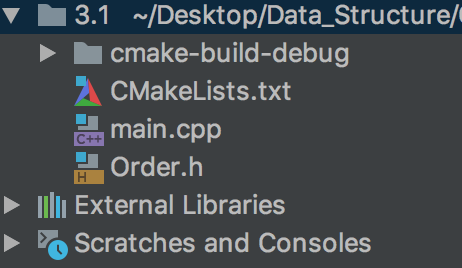
\includegraphics[width=0.8\textwidth]{project31.png}
\end{figure}

2.依次点击菜单"Run"->build,再点击"Run",程序就执行六种排序算法

\section{测试结果}

程序生成随机数据后自动执行六种排序算法,并将五轮生成的随机数个
数和各种排序算法的比较次数和移动次数打印在屏幕上。
\begin{figure}[h]
    \centering
    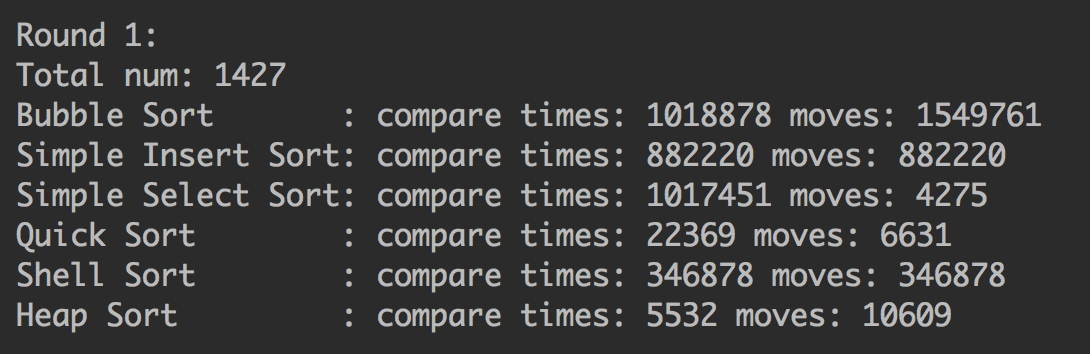
\includegraphics[width=0.8\textwidth]{result.png}
\end{figure}

	根据以上测试结果数据分析,可以得出模拟数据与理论时间复杂度相符。

\section{附录}

源程序文件名清单

main.cpp               \qquad \quad  //主函数

Order.h            \qquad \qquad //排序函数单元模块



\end{document}




